\documentclass[a4paper]{scrreprt}
\usepackage[german]{babel}
\usepackage[utf8]{inputenc}
\usepackage[T1]{fontenc}
\usepackage{graphicx}
\graphicspath{ {images/} }
\usepackage{ae}

\begin{document}
    \chapter{Anwendungsfälle}
    		\begin{figure}[h]
			\centering
			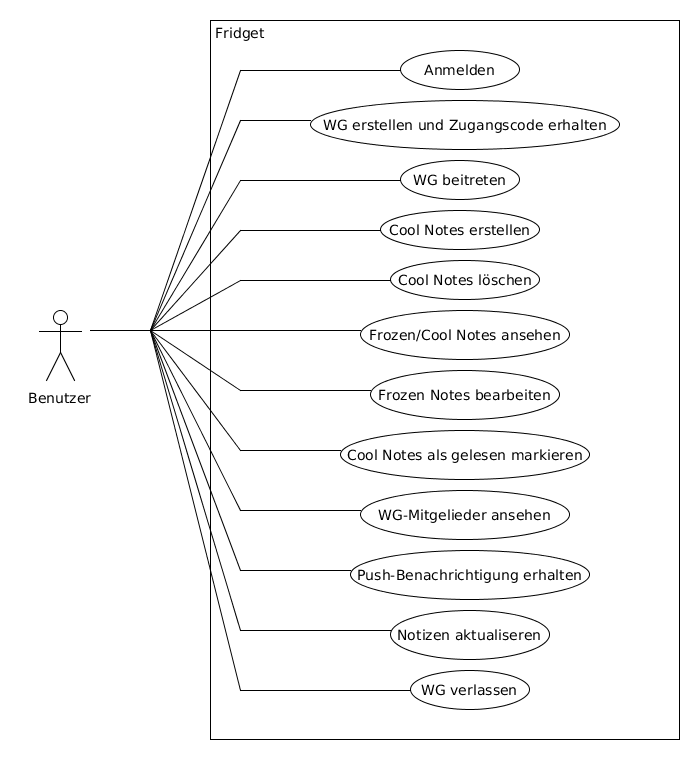
\includegraphics[scale = .6]{anwendungsfalldiagramm.png}
			\caption{Anwendungsfalldiagramm}
		\end{figure}
    		    		
        \section{Anmelden}
        \textbf{Teilnehmende Akteure}: Benutzer \\
		\textbf{Eingangsbedingungen}: Der Benutzer hat Fridget installiert und besitzt ein Google-Konto. Das Internet ist verfügbar. \\
		\textbf{Ausgangsbedingung}: Der Benutzer hat sich angemeldet. \\
		\textbf{Ereignisfluss}: Benutzer wird angemeldet
		
		\section{WG erstellen und Zugangscode erhalten}
		\textbf{Teilnehmende Akteure}: Benutzer \\
		\textbf{Eingangsbedingungen}: Der Benutzer hat sich angemeldet. Das Internet ist verfügbar. \\
		\textbf{Ausgangsbedingung}: Ein Zugangscode wurde angezeigt. \\
		\textbf{Ereignisfluss}: WG wird erstellt $\rightarrow$ Zugangscode wird generiert
		
		\section{WG beitreten}
		\textbf{Teilnehmende Akteure}: Benutzer \\
		\textbf{Eingangsbedingungen}: Der Benutzer hat sich angemeldet und besitzt einen gültigen Zugangscode. Die WG ist nicht voll. Das Internet ist verfügbar. \\
		\textbf{Ausgangsbedingung}: Der Benutzer ist einer WG beigetreten. \\
		\textbf{Ereignisfluss}: WG wird beigetreten
		
		\section{Cool Notes erstellen}
		\textbf{Teilnehmende Akteure}: Benutzer \\
		\textbf{Eingangsbedingungen}: Der Benutzer hat sich angemeldet und ist einer WG beigetreten. Die Pinnwand ist nicht voll und keiner erstellt gerade die letzte Cool Note. Das Internet ist verfügbar. \\
		\textbf{Ausgangsbedingung}: Der Benutzer hat das Erstellen bestätigt. \\
		\textbf{Ereignisfluss}: Cool Note wird erstellt
		
		\section{Cool Notes löschen}
		\textbf{Teilnehmende Akteure}: Benutzer \\
		\textbf{Eingangsbedingungen}: Der Benutzer hat eine Cool Note, die nicht von ihm erstellt wurde, geöffnet. Keiner liest gerade dieselbe Cool Note. Das Internet ist verfügbar. \\
		\textbf{Ausgangsbedingung}: Der Benutzer hat das Löschen bestätigt. \\
		\textbf{Ereignisfluss}: Cool Note wird gelöscht
		
		\section{Frozen/Cool Notes ansehen}
		\textbf{Teilnehmende Akteure}: Benutzer \\
		\textbf{Eingangsbedingungen}: Der Benutzer hat sich angemeldet und ist einer WG beigetreten. Die Pinnwand ist nicht leer. Das Internet ist verfügbar. \\
		\textbf{Ausgangsbedingung}: Eine Frozen/Cool Note wurde angezeigt. \\
		\textbf{Ereignisfluss}: Frozen/Cool Note wird geöffnet $\rightarrow$ Frozen/Cool Note wird angesehen
		
		\section{Frozen Notes bearbeiten}
		\textbf{Teilnehmende Akteure}: Benutzer \\
		\textbf{Eingangsbedingungen}: Der Benutzer hat eine Frozen Note geöffnet. Keiner bearbeitet gerade dieselbe Frozen Note. Das Internet ist verfügbar. \\
		\textbf{Ausgangsbedingung}: Der Benutzer hat das Bearbeiten bestätigt. \\
		\textbf{Ereignisfluss}: Frozen Note wird bearbeitet
		
		\section{Cool Notes als gelesen markieren}
		\textbf{Teilnehmende Akteure}: Benutzer \\
		\textbf{Eingangsbedingungen}: Der Benutzer hat eine Cool Note, die nicht von ihm erstellt wurde, geöffnet. Die Cool Note wurde noch nicht als gelesen markiert. Das Internet ist verfügbar. \\
		\textbf{Ausgangsbedingung}: Der Benutzer hat die Cool Note als gelesen markiert. \\
		\textbf{Ereignisfluss}: Cool Note wird markiert
		
		\section{WG-Mitgelieder ansehen}
		\textbf{Teilnehmende Akteure}: Benutzer \\
		\textbf{Eingangsbedingungen}: Der Benutzer hat sich angemeldet und ist einer WG beigetreten. Das Internet ist verfügbar. \\
		\textbf{Ausgangsbedingung}: Die WG-Mitgelieder werden angezeigt. \\
		\textbf{Ereignisfluss}: WG-Mitgelieder-View wird geöffnet $\rightarrow$ WG-Mitgelieder werden angesehen
		
		\section{Push-Benachrichtigung erhalten}
		\textbf{Teilnehmende Akteure}: Benutzer \\
		\textbf{Eingangsbedingungen}: Der Benutzer hat sich angemeldet und ist einer WG beigetreten. Der Benutzer hat ``Push-Benachrichtigung'' von Fridget aktiviert. Das Internet ist verfügbar. \\
		\textbf{Ausgangsbedingung}: Die Push-Benachrichtigung wird auf den Geräten des Benutzers angezeigt. \\
		\textbf{Ereignisfluss}: Neue Cool Note wird erstellt $\rightarrow$ Push-Benachrichtigung wird erhalten
		
		\section{Notizen/Mitglieder aktualisieren}
		\textbf{Teilnehmende Akteure}: Benutzer \\
		\textbf{Eingangsbedingungen}: Der Benutzer hat sich angemeldet und ist einer WG beigetreten. Das Internet ist verfügbar. \\
		\textbf{Ausgangsbedingung}: Die Änderungen von Notizen/Mitgliedern wurden mit dem Server synchronisiert. \\
		\textbf{Ereignisfluss}: Pinnwand wird nach unten gewischt $\rightarrow$ Notizen/Mitglieder werden aktualisiert
		
		\section{WG verlassen}
		\textbf{Teilnehmende Akteure}: Benutzer \\
		\textbf{Eingangsbedingungen}: Der Benutzer hat sich angemeldet und ist einer WG beigetreten. Das Internet ist verfügbar. \\
		\textbf{Ausgangsbedingung}: Der Benutzer hat das Verlassen der WG bestätigt. \\
		\textbf{Ereignisfluss}: WG wird verlassen
\end{document}